\chapter{Dynamics}\label{chap:dynamics}
This chapter will contain an analysis of the dynamics of the pan/tilt system which will result in a mathematical model. Calculations made throughout this chapter will reside in appendix \ref{app:dynamics_calc}. Identifying and understanding the relevant dynamics of a system is important as this will lead to an as accurate theoretical model as needed for the application. Ideally a perfect model would somewhat be preferred, but it would be a very difficult and tedious task to derive a perfect model and completely unnecessary to achieve. The reason for that is some of the dynamics are completely insignificant to the behaviour of the system, some other might have a little impact on the behaviour but can be omitted due to more dominating dynamic. The response of electrical circuits are often much quicker than the response of a mechanical system. This response delay is encoded into the poles of a system, which makes the poles of the system very interesting to analyse. The poles of the system tell if it is stable, and if any dynamic in the system possibly can be omitted due to its relatively fast response compared to the rest of the system which acts slower.

%Every system can be constructed of first order systems and second order systems in a cascade. These two types of systems defines a time constant. For first order systems this time constant is hidden in the zeroth order term and in second order systems it is hidden in the first order term. The time constant defines $ 1 - \sfrac{1}{e} \approx 63.2% $ of its energy level. 

\section{Overview of pan/tilt}
The following will give an overview of the physical aspects of the pan/tilt system and also define the mathematics which is tied to the system. The pan/tilt is assembled from two motors, a set of gears connected to each motor. Each motor can rotate a mass individually by transferring torque from the motors, through the gears, to the masses which are connected to the gears. A model of the motors are needed, along with a model of the reflected inertia through the gears, and other dynamics might be relevant to, but are discussed later in this section.

\subsection{Motor}
The motor converts electrical energy to mechanical energy as a voltage is supplied to the motor. This voltage make the motor turn and this turning motion deliver torque though some gears to a mass which then spins up to some maximum speed. A simplification of a DC motors circuit can be seen in figure \ref{fig:motor_circuit}, from this a mathematical model of the motor can be derived.
\begin{figure}[htb]
	\begin{center}
	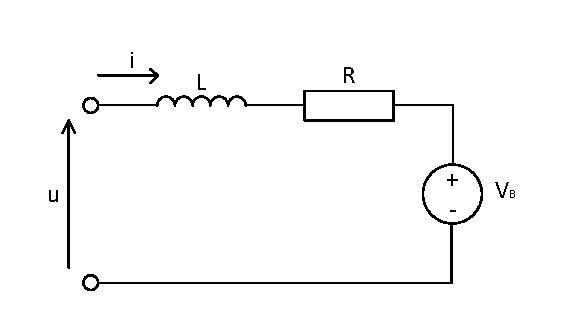
\includegraphics[scale=1,trim=0 0 0 0]{graphics/motor_circuit.pdf} %trim=l b r t (can cut off from every side)
	\caption{Simplification of circuit for a DC motor. Voltage supplied is denoted by $u$, $i$ is the current through the motor, $L$ is inductance, $R$ is resistance and $V_B$ is the the voltage generated from the coil rotating in a magnetic field.}
	\label{fig:motor_circuit}			% figure labels are of the form \label{fig:*}
	\end{center}
\end{figure}
Following can be derived from the circuit seen in figure \ref{fig:motor_circuit}.
\begin{align}
	u &= L\frac{di}{dt} +  Ri + V_B \Longleftrightarrow\\
	u &= L\frac{di}{dt} +  Ri + K_B\omega\label{eq:motor_model}
\end{align}
where $u$ is the voltage input, $i$ is the current, $\frac{di}{dt}$ is the time derivative of the current, $L$ is the inductance, $R$ is the resistance and $V_B$ is the voltage generated in the in coil of the motor as it spins in a magnetic field. $V_B$ can be expressed by $K_B$ which is the \textit{back-emf}\footnote{EMF is an abbreviation for electromotive force, which is the voltage generated from a coil rotating in a magnetic field.}-constant, times $\omega$, which is the angular velocity of the motor. As the motors need to move a mass an expression for torque is more interesting compared to the expression derived in \ref{eq:motor_model}. The electrical torque can be expressed in the following way:
\begin{equation}
	\tau = K_Ti\label{eq:electrical_torque}
\end{equation}
where $K_T$ is the torque constant.	The mechanical torque can be expressed in the following way:
\begin{equation}
	\tau = J_L\frac{d\omega}{dt}\label{eq:mechanical_torque}
\end{equation}
where $J_L$ is the inertial load on the motor, $\frac{d\omega}{dt}$ is the time derivative of the angular velocity of the motor. Equation \ref{eq:electrical_torque} and \ref{eq:mechanical_torque} equals each other if it is assumed that the energy is conserved in the transfer from electrical to mechanical torque, the following expression is obtained then obtained from equation \ref{eq:electrical_torque} and \ref{eq:mechanical_torque}:
\begin{align}
	K_Ti &= J_L\frac{d\omega}{dt} \Leftrightarrow\\
	i &= \frac{J_L}{K_T} \frac{d\omega}{dt}\label{eq:electrical_mechanical_torque}
\end{align}
To derive $\frac{di}{dt}$ the time derivative is taken of \ref{eq:electrical_mechanical_torque} which leads to:
\begin{equation}
	\frac{di}{dt} = \frac{J_L}{K_T} \frac{d^{2}\omega}{dt^{2}}\label{eq:electrical_mechanical_torque_derivative}
\end{equation}
Now \ref{eq:electrical_mechanical_torque} and \ref{eq:electrical_mechanical_torque_derivative} can be substituted into \ref{eq:motor_model} in which the following is obtained:
\begin{equation}
	u = \frac{L J_L}{K_T} \frac{d^{2}\omega}{dt^{2}} + \frac{R J_L}{K_T} \frac{d\omega}{dt} + K_B \omega
\end{equation}
%An expression for torque is needed, so the above equation is rewritten with respect to \ref{eq:mechanical_torque} which subsequently leads to:
%\begin{equation}
%	J_L \frac{d\omega}{dt} = \frac{K_T}{R} u - \frac{L J_L}{R} \frac{d^{2}\omega}{dt^{2}} - \frac{K_B K_T}{R} \omega\label{eq:torque_motor_model}
%\end{equation}

Stiction, coulomb and viscous friction are omitted as it is assumed that the inertia from the internal friction of the motor is a lot less than the inertia from the mass, so this concludes the model of the motor.

\subsection{Gears}
The gears does not add to the dynamics of the system but changes the existing poles of the existing system. Calculations for reflected inertia is kept in \ref{app:dynamics_calc}. 
  
\subsection{Precession}

\subsection{Omitted dynamic}

\section{State space}